\documentclass{ximera}

\input{preamble.tex}

\author{Gregory Hartman \and Matthew Carr}
\license{Creative Commons 3.0 By-NC}
\acknowledgement{https://github.com/APEXCalculus}

\begin{document}
\begin{exercise}

\outcome{Calculate limits using the limit laws.}
\outcome{Calculate the limit as $x$ approaches $\pm\infty$ of common functions algebraically.}
\outcome{Find the limit as x approaches $\pm\infty$ from a graph.}


Let $f(x) = 2^x+10$. Find
\begin{enumerate}
\item		$\lim_{x\to -\infty} f(x)\begin{prompt} = \answer{10}\end{prompt}$
\item		$\lim_{x\to \infty} f(x)\begin{prompt} = \answer{\infty}\end{prompt}$
\end{enumerate}

\begin{center}
\noindent\begin{minipage}[t]{.5\linewidth}
 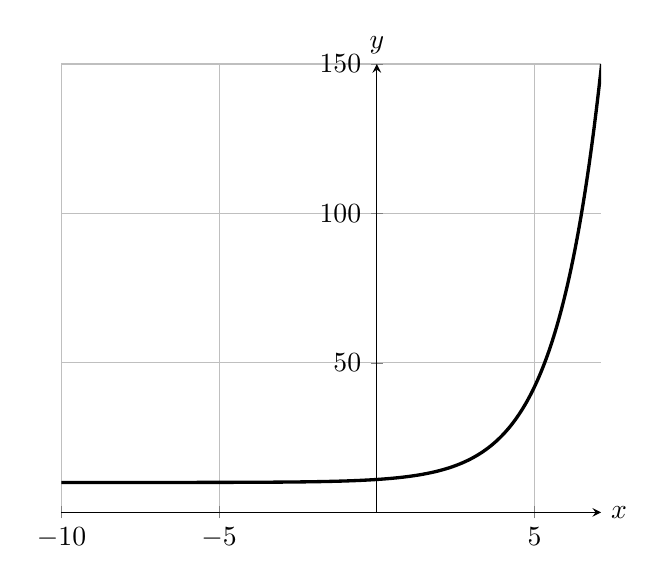
\begin{tikzpicture}
	\begin{axis}
	[ymin=0,ymax=150, axis lines=center,xlabel=$x$,ylabel=$y$,every axis y 
	label/.style={at=(current axis.above origin),anchor=south},every axis x label/.style={at=(current axis.right of origin),anchor=west},
	domain=-1:2,
	ytick={50,100,150},
	yticklabels={$50$,$100$,$150$},
	xtick={-10,-5,5},
	xticklabels={$-10$,$-5$,$5$},
	ymajorgrids=true,
	grid = major
	]
	\addplot[domain=-10:7.13,very thick,smooth,samples=1000]
	{pow(2,\x)+10};
	\end{axis}
       \end{tikzpicture}
\end{minipage}
\end{center}


\end{exercise}
\end{document}